\documentclass[11pt,a4paper]{article}

\usepackage[T1]{fontenc}
\usepackage[utf8]{inputenc}
\usepackage{lmodern}
\usepackage{microtype}
\usepackage{geometry}
\geometry{margin=2.2cm}

\usepackage{graphicx}
\usepackage{booktabs}
\usepackage{longtable}
\usepackage{enumitem}
\usepackage{float}
\usepackage{hyperref}
\hypersetup{colorlinks=true, linkcolor=blue, urlcolor=blue, citecolor=blue}

\title{Understanding and Detecting Malicious Prompts\\
Using Embeddings, Clustering, and Classification\\
\large{FoDS Project Report}}
\author{Krzysztof Knap}
\date{\today}


% --- Figure placeholder macro (keeps space in the PDF even if images are not embedded) ---
% Usage: \FigPlaceholder{EXPORT_NAME}{CAPTION_TEXT}{fig:label}
\newcommand{\FigPlaceholder}[3]{%
\begin{figure}[hbtp]
  \centering
  \fbox{%
    \parbox[c][0.33\textheight][c]{0.92\linewidth}{%
      \centering
      \textbf{PLACEHOLDER IMAGE}\\[0.4em]
      \texttt{\detokenize{#1}}\\[0.8em]
      \footnotesize #2
    }%
  }
  \caption{#2 \;(\texttt{\detokenize{#1}})}
  \label{#3}
\end{figure}
}

% --- Inline code macro (safe for underscores) ---
\newcommand{\Code}[1]{\texttt{\detokenize{#1}}}

\begin{document}
\maketitle

\begin{abstract}
We analyze the PL-Guard dataset of Polish prompts using a pretrained multilingual sentence embedding model. We reduce dimensions (PCA, t-SNE, UMAP), test clustering (K-Means, Agglomerative, DBSCAN, HDBSCAN), detect outliers, and train simple classifiers (Logistic Regression, Linear SVM, Random Forest). We also check robustness on adversarial edits. In short: clustering finds only part of the 15-class structure, some classes are always mixed, and classifiers drop in performance on adversarial text. Adding a small amount of adversarial data to training improves robustness.
\end{abstract}

\section{Project scope}
This report summarizes results from a Fundamentals of Data Science project based on the PL-Guard dataset (malicious prompt analysis). The goal is educational: to practice embeddings, dimensionality reduction, interactive visualization, clustering, outlier detection, and supervised learning, and to study robustness under adversarial text perturbations.
\newline Simple takeaway: the report focuses on learning methods, not on building a production system.

\section{Dataset and preprocessing}
\textbf{Dataset.} The notebook uses PL-Guard from Hugging Face, with a \texttt{test} split of \textbf{900} prompts and \textbf{15} categories (one \texttt{safe} class and multiple \texttt{unsafe\textbackslash nS\#} subcategories). An adversarial split (\texttt{test\_adversarial}) provides modified versions of the same prompts.

\textbf{Schema.} The dataset splits contain:
\begin{itemize}[leftmargin=*]
\item \texttt{test}: \texttt{text}, \texttt{category}
\item \texttt{test\_adversarial}: \texttt{original\_text}, \texttt{category}, \texttt{text}, \texttt{num\_changes}, \texttt{modification\_types}
\end{itemize}

\textbf{Class balance.} The data are nearly balanced across unsafe subcategories, with one larger safe class:
\begin{center}
\begin{tabular}{lrr}
\toprule
Category & Count & Share \\
\midrule
\texttt{safe} & 200 & 0.2222 \\
\texttt{unsafe\textbackslash nS1}  & 50 & 0.0556 \\
\texttt{unsafe\textbackslash nS2}  & 50 & 0.0556 \\
\texttt{unsafe\textbackslash nS3}  & 50 & 0.0556 \\
\texttt{unsafe\textbackslash nS4}  & 50 & 0.0556 \\
\texttt{unsafe\textbackslash nS5}  & 50 & 0.0556 \\
\texttt{unsafe\textbackslash nS6}  & 50 & 0.0556 \\
\texttt{unsafe\textbackslash nS7}  & 50 & 0.0556 \\
\texttt{unsafe\textbackslash nS8}  & 50 & 0.0556 \\
\texttt{unsafe\textbackslash nS9}  & 50 & 0.0556 \\
\texttt{unsafe\textbackslash nS10} & 50 & 0.0556 \\
\texttt{unsafe\textbackslash nS11} & 50 & 0.0556 \\
\texttt{unsafe\textbackslash nS12} & 50 & 0.0556 \\
\texttt{unsafe\textbackslash nS13} & 50 & 0.0556 \\
\texttt{unsafe\textbackslash nS14} & 50 & 0.0556 \\
\bottomrule
\end{tabular}
\end{center}

\textbf{Basic quality checks.} The \texttt{text} field has \textbf{0} empty/None entries in the \texttt{test} split.

\textbf{Preprocessing.} Because we rely on a pretrained sentence embedding model, preprocessing is intentionally minimal. Prompts are used as-is after basic inspection of dataset columns. Embeddings are computed with L2 normalization enabled, which makes cosine distance a natural measure of semantic change and improves comparability across samples. In high-dimensional text settings, this approach is common: most of the signal comes from the pretrained encoder rather than handcrafted cleaning rules.
\newline Simple takeaway: we keep text almost unchanged, so results mostly come from the embedding model, not from heavy cleaning.

\section{Text representation with embeddings}
Prompts are embedded using a pretrained multilingual sentence-transformer:
\begin{itemize}[leftmargin=*]
\item Model: \texttt{sentence-transformers/paraphrase-multilingual-MiniLM-L12-v2}
\item Embedding dimensionality: \textbf{384}
\item Normalization: L2-normalized embeddings (cosine similarity/distance becomes a natural metric)
\end{itemize}

\noindent\textbf{Why normalization matters.} With normalized vectors, cosine distance focuses on semantic direction rather than raw magnitude. This simplifies comparisons between original vs adversarial prompts and improves the stability of downstream methods that rely on distance geometry.
\newline Simple takeaway: normalization makes distances easier to compare across samples.

\section{Dimensionality reduction and visualization}
We use PCA, t-SNE, and UMAP to reduce embeddings to 2D for visualization and qualitative analysis.

\subsection{PCA}
PCA provides a fast linear projection that is easy to interpret, but it often cannot fully separate complex semantic classes.
In this dataset, PCA explains a limited amount of variance: \textbf{14.22\%} with 2 components and \textbf{19.70\%} with 3 components. This is expected for high-dimensional sentence embeddings.
Simple conclusion: PCA loses a lot of information in 2D/3D, so it is good for a quick overview, not for clean separation of categories.

\begin{figure}[htbp]
  \centering
  \includegraphics[width=0.95\linewidth]{figures/s1.png}
  \caption{PCA 2D scatter of embeddings colored by category}
  \label{fig:dbscan1}
\end{figure}

\subsection{t-SNE}
t-SNE is nonlinear and often forms visually compact groups, but it can distort global geometry. The notebook compares:
\begin{itemize}[leftmargin=*]
\item end-to-end t-SNE directly from 384D embeddings,
\item PCA(50) $\rightarrow$ t-SNE,
\item PCA(150) $\rightarrow$ t-SNE.
\end{itemize}

\begin{figure}[htbp]
  \centering
  \includegraphics[width=0.95\linewidth]{figures/s2.png}
  \caption{t-SNE scatter (384$\rightarrow$2D) colored by category}
  \label{fig:dbscan1}
\end{figure}
\begin{figure}[htbp]
  \centering
  \includegraphics[width=0.95\linewidth]{figures/s3.png}
  \caption{t-SNE scatter (PCA50$\rightarrow$t-SNE) colored by category}
  \label{fig:dbscan1}
\end{figure}
\begin{figure}[htbp]
  \centering
  \includegraphics[width=0.95\linewidth]{figures/s4.png}
  \caption{t-SNE scatter (PCA150$\rightarrow$t-SNE) colored by category}
  \label{fig:dbscan1}
\end{figure}

To quantify neighborhood preservation, the notebook reports \textbf{trustworthiness} at multiple neighborhood sizes $k$:

\begin{center}
\begin{tabular}{lccc}
\toprule
Method & $k=5$ & $k=10$ & $k=20$ \\
\midrule
t-SNE (384$\rightarrow$2D) & 0.9532 & 0.9293 & 0.9045 \\
PCA50$\rightarrow$t-SNE (end-to-end 384$\rightarrow$2D) & 0.9646 & 0.9419 & 0.9189 \\
PCA150$\rightarrow$t-SNE (end-to-end 384$\rightarrow$2D) & 0.9559 & 0.9327 & 0.9070 \\
\bottomrule
\end{tabular}
\end{center}

Interpretation: PCA50$\rightarrow$t-SNE preserves local neighborhoods slightly better than running t-SNE directly on 384D. This supports using PCA as a denoising step before t-SNE.
Simple conclusion: t-SNE shows local similarity well, but distances between far-apart groups on the plot are not reliable.


\subsection{UMAP}
UMAP is another nonlinear technique that often balances local and global structure well. Trustworthiness results for UMAP 2D are:

\begin{center}
\begin{tabular}{lccc}
\toprule
Method & $k=5$ & $k=10$ & $k=20$ \\
\midrule
UMAP (384$\rightarrow$2D) & 0.9478 & 0.9141 & 0.8739 \\
\bottomrule
\end{tabular}
\end{center}
Simple conclusion: UMAP is a reasonable compromise between local structure and global layout, but it still cannot fully separate all 15 labels.

\begin{figure}[htbp]
  \centering
  \includegraphics[width=0.95\linewidth]{figures/s5.png}
  \caption{UMAP 2D scatter colored by category; hover tooltip shows prompt text}
  \label{fig:dbscan1}
\end{figure}


\section{Selected results and discussion: clustering and structure}
All clustering methods are applied to PCA-50 embeddings with L2 normalization (denoted \Code{X_cluster} in the notebook). This reduces noise and keeps distances comparable.
Simple takeaway: we cluster in a lower-dimensional space to get more stable results.

To evaluate clustering quality beyond global purity/silhouette, we report:
\begin{itemize}[leftmargin=*]
\item \textbf{Category mixing (entropy).} For each true category, we check how its samples are spread across clusters. Higher entropy means the category is split across many clusters (more mixed). We also report the \textbf{dominant share}, i.e., the fraction of that category that falls into its biggest cluster (the cluster that contains the most samples from that category).
\item \textbf{Cluster coherence (purity).} For each cluster, purity is the dominant true-category fraction inside the cluster. High purity indicates a coherent cluster.
\item \textbf{Distance metric note.}  We use Euclidean distance for clustering and outlier detection because it is the default geometry assumed by K-Means and Ward linkage, and it is also natural for density-based methods when operating in a vector space. For adversarial analysis we report cosine distance, because it directly measures semantic direction change in embedding space. Importantly, embeddings are L2-normalized, so for normalized vectors Euclidean distance is a monotonic transform of cosine distance ($\|x-y\|^2 = 2(1-\cos)$), meaning neighborhood rankings are consistent across both metrics; cosine is used mainly for interpretability.
\end{itemize}

\subsection{K-Means (k=15)}
\begin{itemize}[leftmargin=*]
\item \textbf{Purity (K-Means, $k=15$):} $\approx 0.571$
\item \textbf{Silhouette:} low ($\approx 0.06$--$0.10$)
\end{itemize}
Comment: purity around 0.57 means the clusters only partly match the true labels. The low silhouette confirms that clusters overlap a lot in embedding space, so separation is weak.

\begin{figure}[htbp]
  \centering
  \includegraphics[width=1.0\linewidth]{figures/s6.png}
  \caption{Elbow curve (inertia vs $k$)}
  \label{fig:dbscan1}
\end{figure}
\begin{figure}[hbtp]
    \centering
    \includegraphics[width=1\linewidth]{figures/s7.png}
    \caption{t-SNE scatter colored by K-Means cluster}
    \label{fig:placeholder}
\end{figure}
\begin{figure}[hbtp]
    \centering
    \includegraphics[width=1\linewidth]{figures/s8.png}
    \caption{t-SNE scatter colored by true category}
    \label{fig:placeholder}
\end{figure}


\textbf{Mixing/coherence (K-Means).}
Most mixed: \texttt{unsafe\textbackslash nS2} (entropy$\approx 3.37$, dominant share$\approx 0.18$) and \texttt{safe} (entropy$\approx 2.81$, dominant share$\approx 0.44$).
Most coherent: \texttt{unsafe\textbackslash nS9} (dominant share$\approx 0.90$) and \texttt{unsafe\textbackslash nS10} (dominant share$\approx 0.82$).
Cluster purities range from very high ($\approx 0.99$) to very low ($\approx 0.23$--$0.40$), so the structure is uneven.

\subsection{Agglomerative clustering (Ward, k=15)}
\begin{itemize}[leftmargin=*]
\item \textbf{Purity (Agglomerative, $k=15$):} $\approx 0.539$
\item \textbf{Silhouette:} very low (\textbf{0.0787})
\end{itemize}
Comment: purity is slightly lower than K-Means, so label alignment is even weaker. The very low silhouette again shows that clusters are not well separated.

\begin{figure}[hbtp]
    \centering
    \includegraphics[width=1\linewidth]{figures/s9.png}
    \caption{t-SNE scatter colored by Agglomerative clusters (Ward, $k=15$)}
    \label{fig:placeholder}
\end{figure}


\textbf{Mixing/coherence (Agglomerative).}
Most mixed: \texttt{unsafe\textbackslash nS2} (entropy$\approx 3.11$, dominant share$\approx 0.18$) and \texttt{unsafe\textbackslash nS6} (entropy$\approx 2.71$, dominant share$\approx 0.40$); \texttt{safe} is also spread out.
Most coherent: \texttt{unsafe\textbackslash nS13} (dominant share$\approx 0.78$) and \texttt{unsafe\textbackslash nS9} (dominant share$\approx 0.70$).
Cluster purities range from very high ($\approx 0.99$) to very low ($\approx 0.18$--$0.38$).

\subsection{DBSCAN (excluding noise)}
Because DBSCAN often labels many points as noise in reduced/normalized space, we report mixing/coherence \emph{excluding} noise points.
\subsubsection{}
\begin{figure}[hbtp]
    \centering
    \includegraphics[width=1\linewidth]{figures/s10.png}
    \caption{k-distance plot used to choose DBSCAN eps}
    \label{fig:placeholder}
\end{figure}
\begin{figure}[hbtp]
    \centering
    \includegraphics[width=1\linewidth]{figures/s11.png}
    \caption{DBSCAN result scatter: color=cluster, highlight noise/outliers}
    \label{fig:placeholder}
\end{figure}


\paragraph{Parameter search and justification.}
A coarse grid search over \texttt{eps} and \texttt{min\_samples} shows that the commonly tried range
\texttt{eps=0.55--0.70} is ineffective here: most configurations label nearly the entire dataset as noise (e.g., at \texttt{eps=0.55} about 95\% are outliers, and even at \texttt{eps=0.70, min\_samples=3} about 68\% remain outliers).
More meaningful behavior emerges only around \texttt{eps=0.75--0.80}, where outliers decrease (e.g., \texttt{517} $\rightarrow$ \texttt{409}) and the number of clusters drops (e.g., \texttt{38} $\rightarrow$ \texttt{32}), indicating cluster merging---a typical DBSCAN trade-off: larger \texttt{eps} reduces noise but risks merging distinct groups.



\textbf{Mixing/coherence (DBSCAN; excluding noise).}
Most mixed: \texttt{unsafe\textbackslash nS2} and \texttt{unsafe\textbackslash nS7} (dominant share$\approx 0.45$--$0.50$).
Most coherent: \texttt{unsafe\textbackslash nS9}/\texttt{unsafe\textbackslash nS10}/\texttt{unsafe\textbackslash nS14} (dominant share$=1.00$ among non-noise).
There is one very large mixed cluster (size 225, purity$\approx 0.36$), plus many tiny pure clusters.
Comment: DBSCAN can create very pure small clusters, but overall structure is uneven because a large mixed cluster dominates. Silhouette is not reported here because DBSCAN has many noise points and non-spherical clusters, so silhouette is less informative.

\subsection{HDBSCAN (min\_cluster\_size=10, min\_samples=1; excluding outliers)}
HDBSCAN adaptively chooses density levels and explicitly identifies outliers; we summarize results \emph{excluding} outliers: clusters=14, outliers=414

\begin{figure}[hbtp]
    \centering
    \includegraphics[width=1\linewidth]{figures/s19.png}
    \caption{HDBSCAN cluster scatter highlighting outliers}
    \label{fig:placeholder}
\end{figure}

\textbf{Mixing/coherence (HDBSCAN; excluding outliers).}
Most mixed: \texttt{unsafe\textbackslash nS2} (dominant share$\approx 0.22$) and \texttt{safe} (dominant share$\approx 0.44$).
Most coherent: \texttt{unsafe\textbackslash nS10} and \texttt{unsafe\textbackslash nS9} (dominant share$=1.00$), with \texttt{unsafe\textbackslash nS13}/\texttt{unsafe\textbackslash nS5}/\texttt{unsafe\textbackslash nS11} also strong.
Cluster purities still range widely (down to $\approx 0.30$--$0.37$).
Comment: HDBSCAN finds clear cores for some labels (high purity), but many points become outliers or end up in mixed clusters. Silhouette is not reported because HDBSCAN produces variable-density clusters and many outliers, so silhouette is not a stable summary here.

\subsection{Overall interpretation}
Across all four methods, two patterns are stable. First, some categories show clear semantic cores (e.g., \texttt{unsafe\textbackslash nS9}, \texttt{unsafe\textbackslash nS10}) and remain coherent regardless of algorithm. Second, categories like \texttt{safe} and \texttt{unsafe\textbackslash nS2} are repeatedly mixed, suggesting they contain diverse intents or share vocabulary with other labels. Therefore, clustering can reveal useful structure (cores and mixed regions), but it cannot reliably reconstruct the full 15-class ground-truth taxonomy from embeddings alone.

\section{Outlier detection}
We treat noise points from density-based methods as outliers and also define percentile-based ``extreme'' samples.
Simple takeaway: outliers here mean “unusual in embedding space,” not necessarily “most dangerous.”

\subsection{Distance-based outliers in embedding space}
Using a distance-to-centroid approach, the notebook sets a Q95 threshold:
\begin{itemize}[leftmargin=*]
\item \textbf{Distance-to-centroid threshold (Q95):} 1.4314
\item \textbf{Outliers:} 45/900 (\textbf{5\%})
\end{itemize}
We compute the average embedding (the “center” of all points) and measure how far each prompt is from this center. The top 5\% farthest prompts are labeled as outliers, which gives the threshold 1.4314 and 45/900 outliers.
We also see that \texttt{safe} appears more often among these outliers. A simple explanation is that \texttt{safe} covers many different neutral topics, so those prompts are spread out and some end up far from the center.

\begin{figure}[hbtp]
    \centering
    \includegraphics[width=1\linewidth]{figures/s17.png}
    \caption{Distance-to-centroid (cosine) distribution with the Q95 threshold line}
    \label{fig:placeholder}
\end{figure}


\subsection{Density-based outliers (DBSCAN vs HDBSCAN)}
We also treat points labeled as noise by density-based clustering as outliers. A key observation is that
the \emph{absolute} outlier fraction is highly sensitive to the neighborhood radius (DBSCAN \texttt{eps})
and to the density notion (DBSCAN vs HDBSCAN):

\begin{itemize}[leftmargin=*]
\item \textbf{DBSCAN (PCA-50, L2 norm), min\_samples=3:} \texttt{eps=0.75} $\rightarrow$ \textbf{517/900 (57.44\%)} outliers; \texttt{eps=0.80} $\rightarrow$ \textbf{409/900 (45.44\%)} outliers.
\item \textbf{HDBSCAN robustness check:} depending on \texttt{min\_cluster\_size} and \texttt{min\_samples}, outliers are typically in the \textbf{42.78\%--49.44\%} range.
\end{itemize}
In counts, HDBSCAN flags about \textbf{385--445} outliers out of 900, so almost half the data can be labeled as noise.
Simple conclusion: density methods mark a very large part of the dataset as outliers, so they are better for finding a small core than for clean full clustering.

\newline The embedding space is \emph{density-fragmented} - many prompts lie outside stable dense cores.
This is consistent with the k-distance curves having no sharp elbow and only leveling off around \texttt{eps $\approx$ 0.75--0.80}.
Practically, this means density-based ``outlier'' often captures \emph{rarity of formulation/topic/style} rather than ``maliciousness'' per se.

\paragraph{Agreement between methods:}
\newline For one representative HDBSCAN configuration, the intersection of DBSCAN outliers (\texttt{eps=0.75}) and HDBSCAN outliers contains \textbf{437} samples, while the union contains \textbf{590}.
Relative to DBSCAN's 517 outliers, \textbf{80} are flagged only by DBSCAN, and HDBSCAN adds \textbf{73} additional outliers.
This convergence suggests that, despite different density models, both methods identify a stable ``atypical'' subset.

\subsection{Adversarial movement outliers}
For each prompt, original vs adversarial embeddings are compared using cosine distance. The notebook reports:
\begin{itemize}[leftmargin=*]
\item \textbf{Move-cosine threshold (Q95):} 0.6374
\item \textbf{Move-outliers:} 45/900 (\textbf{5\%})
\end{itemize}
The threshold is taken from the data: it is the 95th percentile of all \texttt{move\_cosine} values, so only the top 5\% largest moves are above it.
\newline Simple conclusion: only 5\% of prompts (45/900) cross this threshold (0.6374). So most adversarial edits cause small or moderate shifts, but a small group moves a lot and is most likely to break clustering and classification.
\begin{figure}[hbtp]
    \centering
    \includegraphics[width=1\linewidth]{figures/s20.png}
    \caption{Distribution of adversarial embedding shift (move_cosine) with outlier threshold}
    \label{fig:placeholder}
\end{figure}


\section{Adversarial analysis: what changes and why it matters}
The notebook contains an adversarial split where each original prompt has a modified counterpart. This enables two important checks:
\begin{itemize}[leftmargin=*]
\item \textbf{Semantic stability of embeddings.} If modifications are ``surface-level'', cosine shifts should be small; large shifts suggest that the encoder interprets edits as meaning-changing.
\item \textbf{Robustness of downstream decisions.} Even if semantic shifts are moderate, clustering boundaries and classifier decision margins can be sensitive.
\end{itemize}

\begin{figure}[hbtp]
    \centering
    \includegraphics[width=1\linewidth]{figures/s14.png}
    \caption{Distribution of adversarial cosine shift (move\_cosine)}
    \label{fig:placeholder}
\end{figure}

\begin{figure}[hbtp]
    \centering
    \includegraphics[width=1\linewidth]{figures/s18.png}
    \caption{Cosine shift by modification type (top 6}
    \label{fig:placeholder}
\end{figure}

\begin{figure}[hbtp]
    \centering
    \includegraphics[width=1\linewidth]{figures/s16.png}
    \caption{Adversarial shift vs number of changes (median cosine distance by \Code{num_changes}}
    \label{fig:placeholder}
\end{figure}

\begin{figure}[hbtp]
    \centering
    \includegraphics[width=1\linewidth]{figures/s15.png}
    \caption{Top 20 largest adversarial shifts (cosine distance between original and adversarial embeddings)}
    \label{fig:placeholder}
\end{figure}


\begin{itemize}[leftmargin=*]
\item The histogram of \texttt{move\_cosine} is right-skewed: most edits cause small shifts, but a small tail causes large shifts (Q95 = 0.6374; 45/900 outliers).
\item The boxplot by modification type shows similar shift distributions for the most common edit types, so no single type dominates the effect.
\item The plot of shift vs. \texttt{num\_changes} shows a clear trend: more edits generally mean larger movement in embedding space.
\item The bar chart of the top-20 shifts highlights a few extreme cases that move very far and can break clustering/classification.
\end{itemize}
 Simple takeaway: adversarial edits are a real test of model stability, because even small changes can move a prompt noticeably, and a small subset moves a lot. This motivates explicit evaluation on adversarial data and, if possible, training-time augmentation.

\section{Impact of adversarial changes on clustering}
To test stability, the notebook keeps a fixed K-Means model ($k=15$) trained on original data and predicts clusters for adversarial embeddings projected into the same PCA space:
\begin{itemize}[leftmargin=*]
\item \textbf{Overall cluster switch rate:} \textbf{21.33\%} (192/900)
\end{itemize}
Interpretation: about one in five prompts changes cluster assignment after adversarial edits, so clustering is moderately sensitive to perturbations.

\paragraph{Switch rate vs. number of changes.}
More edits generally imply higher switch rate:
\begin{center}
\begin{tabular}{lr}
\toprule
Num changes (bin) & Switch rate \\
\midrule
1--2 & 0.0132 \\
3--5 & 0.1727 \\
6--10 & 0.1778 \\
11--20 & 0.2761 \\
\bottomrule
\end{tabular}
\end{center}

\paragraph{Switch rate by modification type.}
Among the top 6 most frequent edit types, switches are fairly similar:
\begin{center}
\begin{tabular}{lr}
\toprule
Modification type & Switch rate \\
\midrule
\texttt{swap}      & 0.2622 \\
\texttt{keyboard}  & 0.2619 \\
\texttt{ocr}       & 0.2507 \\
\texttt{delete}    & 0.2504 \\
\texttt{diacritic} & 0.2434 \\
\texttt{insert}    & 0.2415 \\
\bottomrule
\end{tabular}
\end{center}

\begin{table}[htbp]
\centering
\caption{Switch rate by category}
\label{tab:switch-rate-by-category}
\begin{tabular}{lr}
\toprule
\textbf{category} & \textbf{switch\_rate} \\
\midrule
\texttt{unsafe\textbackslash n S1}  & 0.320 \\
\texttt{safe}                     & 0.305 \\
\texttt{unsafe\textbackslash n S2}  & 0.300 \\
\texttt{unsafe\textbackslash n S7}  & 0.280 \\
\texttt{unsafe\textbackslash n S12} & 0.240 \\
\texttt{unsafe\textbackslash n S4}  & 0.220 \\
\texttt{unsafe\textbackslash n S5}  & 0.200 \\
\texttt{unsafe\textbackslash n S3}  & 0.180 \\
\texttt{unsafe\textbackslash n S6}  & 0.160 \\
\texttt{unsafe\textbackslash n S8}  & 0.160 \\
\texttt{unsafe\textbackslash n S13} & 0.160 \\
\texttt{unsafe\textbackslash n S10} & 0.140 \\
\texttt{unsafe\textbackslash n S9}  & 0.140 \\
\texttt{unsafe\textbackslash n S11} & 0.100 \\
\texttt{unsafe\textbackslash n S14} & 0.020 \\
\bottomrule
\end{tabular}
\end{table}


\newpage
\section{Classification and robustness}
We train three baseline classifiers on embeddings (stratified 80/20 split; train=720, test=180; 15 classes):
\begin{itemize}[leftmargin=*]
\item Logistic Regression
\item Linear SVM
\item Random Forest
\end{itemize}
Evaluation uses accuracy and macro-averaged precision/recall/F1.

\subsection{Baseline performance on clean test data}
\begin{center}
\begin{tabular}{lcccc}
\toprule
Model & Accuracy & Precision & Recall & F1-score \\
\midrule
LogReg       & 0.705556 & 0.691059 & 0.666667 & 0.667226 \\
LinearSVM    & 0.677778 & 0.648206 & 0.643333 & 0.637929 \\
RandomForest & 0.683333 & 0.729725 & 0.635000 & 0.652546 \\
\bottomrule
\end{tabular}
\end{center}
Simple conclusion: Logistic Regression is the best baseline on clean data (highest Macro F1), but all models are only moderately accurate.

\subsection{Performance on adversarial test data}
\begin{center}
\begin{tabular}{lcccc}
\toprule
Model & Accuracy$_{\text{adv}}$ & Precision$_{\text{adv}}$ & Recall$_{\text{adv}}$ & F1-score$_{\text{adv}}$ \\
\midrule
LogReg       & 0.611111 & 0.596245 & 0.583333 & 0.579768 \\
LinearSVM    & 0.566667 & 0.550421 & 0.535000 & 0.528370 \\
RandomForest & 0.622222 & 0.677096 & 0.566667 & 0.587483 \\
\bottomrule
\end{tabular}
\end{center}
\noindent Simple conclusion: all models drop on adversarial data, which means small text edits hurt classification.
Among them, Random Forest has the best adversarial Macro F1 (\textbf{0.5875}), but it is still clearly lower than the clean score.

\noindent\textbf{Confusion matrices and clean vs adversarial comparison plots are provided in the Appendix.}

\begin{center}
\begin{tabular}{lcc}
\toprule
Model & Accuracy drop & F1-score drop \\
\midrule
LogReg        & 0.094444 & 0.087458 \\
LinearSVM    & 0.111111 & 0.109559  \\
RandomForest & 0.061111 & 0.065063   \\
\bottomrule
\end{tabular}
\end{center}

\noindent\textbf{Discussion.} The drop from clean to adversarial data shows that model decisions are sensitive to small edits. We use macro metrics because the dataset has many similar-sized unsafe classes and one larger \texttt{safe} class; macro-averaging prevents the large class from hiding errors on smaller classes.

\section{Adversarial augmentation}
The notebook augments training by adding adversarial versions of 30\% of training samples (+216). After augmentation:

\begin{center}
\begin{tabular}{lcccc}
\toprule
Model & Accuracy$_{\text{orig}}$ & Macro-F1$_{\text{orig}}$ & Accuracy$_{\text{adv}}$ & Macro-F1$_{\text{adv}}$ \\
\midrule
LogReg       & 0.716667 & 0.673526 & 0.633333 & 0.598782 \\
LinearSVM    & 0.644444 & 0.597410 & 0.605556 & 0.560615 \\
RandomForest & 0.666667 & 0.633643 & 0.594444 & 0.576239 \\
\bottomrule
\end{tabular}
\end{center}

The augmented training set has \textbf{936} samples (720 original + 216 adversarial).
Simple conclusion: a small amount of adversarial augmentation improves adversarial Macro F1 (e.g., LogReg from 0.5798 to 0.5988) and does not hurt clean accuracy, so the model benefits from seeing these edits during training.


\subsection{Conclusions}
\begin{itemize}[leftmargin=*]
\item \textbf{Clustering is only partly useful.} Some classes have clear cores (e.g., \texttt{unsafe\textbackslash nS9}, \texttt{unsafe\textbackslash nS10}), but many classes mix together, so clustering cannot fully recover all 15 labels.
\item \textbf{Adversarial edits change structure.} Around 21\% of prompts switch clusters after edits, and more edits mean more switches, so the embedding space is not fully stable.
\item \textbf{Supervised models are better but still fragile.} All models lose accuracy on adversarial text; adding 30\% adversarial samples helps, which means the model benefits from seeing these edits during training.
\end{itemize}

\section{Limitations}
\begin{itemize}[leftmargin=*]
\item \textbf{Embedding model is not task-specific.} A general sentence encoder may not separate fine-grained unsafe subcategories well.
\item \textbf{Clustering metrics are imperfect.} Purity can be inflated by many small clusters; silhouette can be low even when structure exists but is not globular.
\item \textbf{Adversarial set definition.} The meaning and severity of adversarial edits depends on how the dataset generates modifications; some edits may be stronger than typical real-world paraphrases.
\item \textbf{Reproducibility.} t-SNE/UMAP and some pipelines are stochastic; fixing seeds and library versions is important for stable figures.
\end{itemize}

\appendix

\section{Additional quantitative details}
\subsection{Adversarial shift vs. cluster switching}
The adversarial cosine shift is much higher for samples that switch clusters:
\begin{center}
\begin{tabular}{lrrrrr}
\toprule
Group & count & mean & median & 75\% & max \\
\midrule
no switch & 708 & 0.1195 & 0.0669 & 0.1616 & 0.9709 \\
switch    & 192 & 0.3943 & 0.3565 & 0.5601 & 1.0161 \\
\bottomrule
\end{tabular}
\end{center}

\subsection{Plots}
\begin{figure}[H]
  \centering
  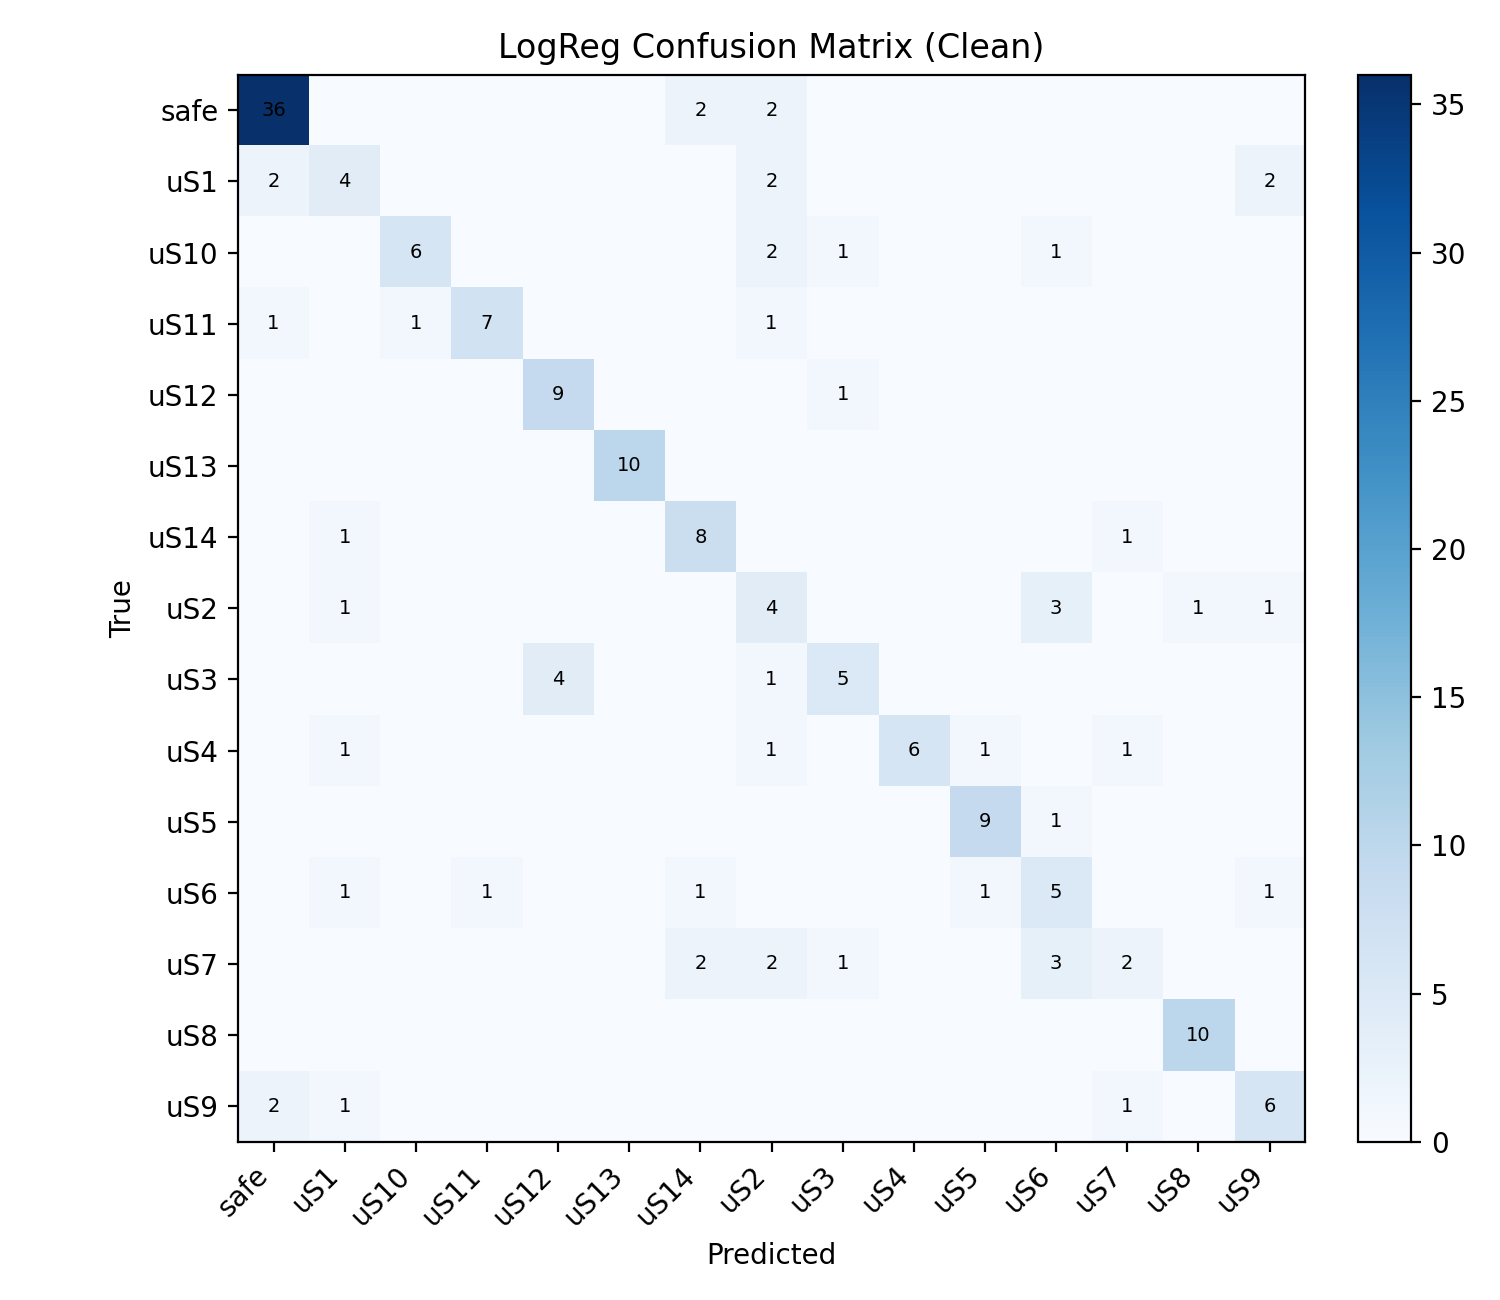
\includegraphics[width=0.8\linewidth]{figures/confusion_logreg_clean.png}
  \caption{Logistic Regression: confusion matrix on clean test set}
  \label{fig:cm-clean}
\end{figure}

\begin{figure}[H]
  \centering
  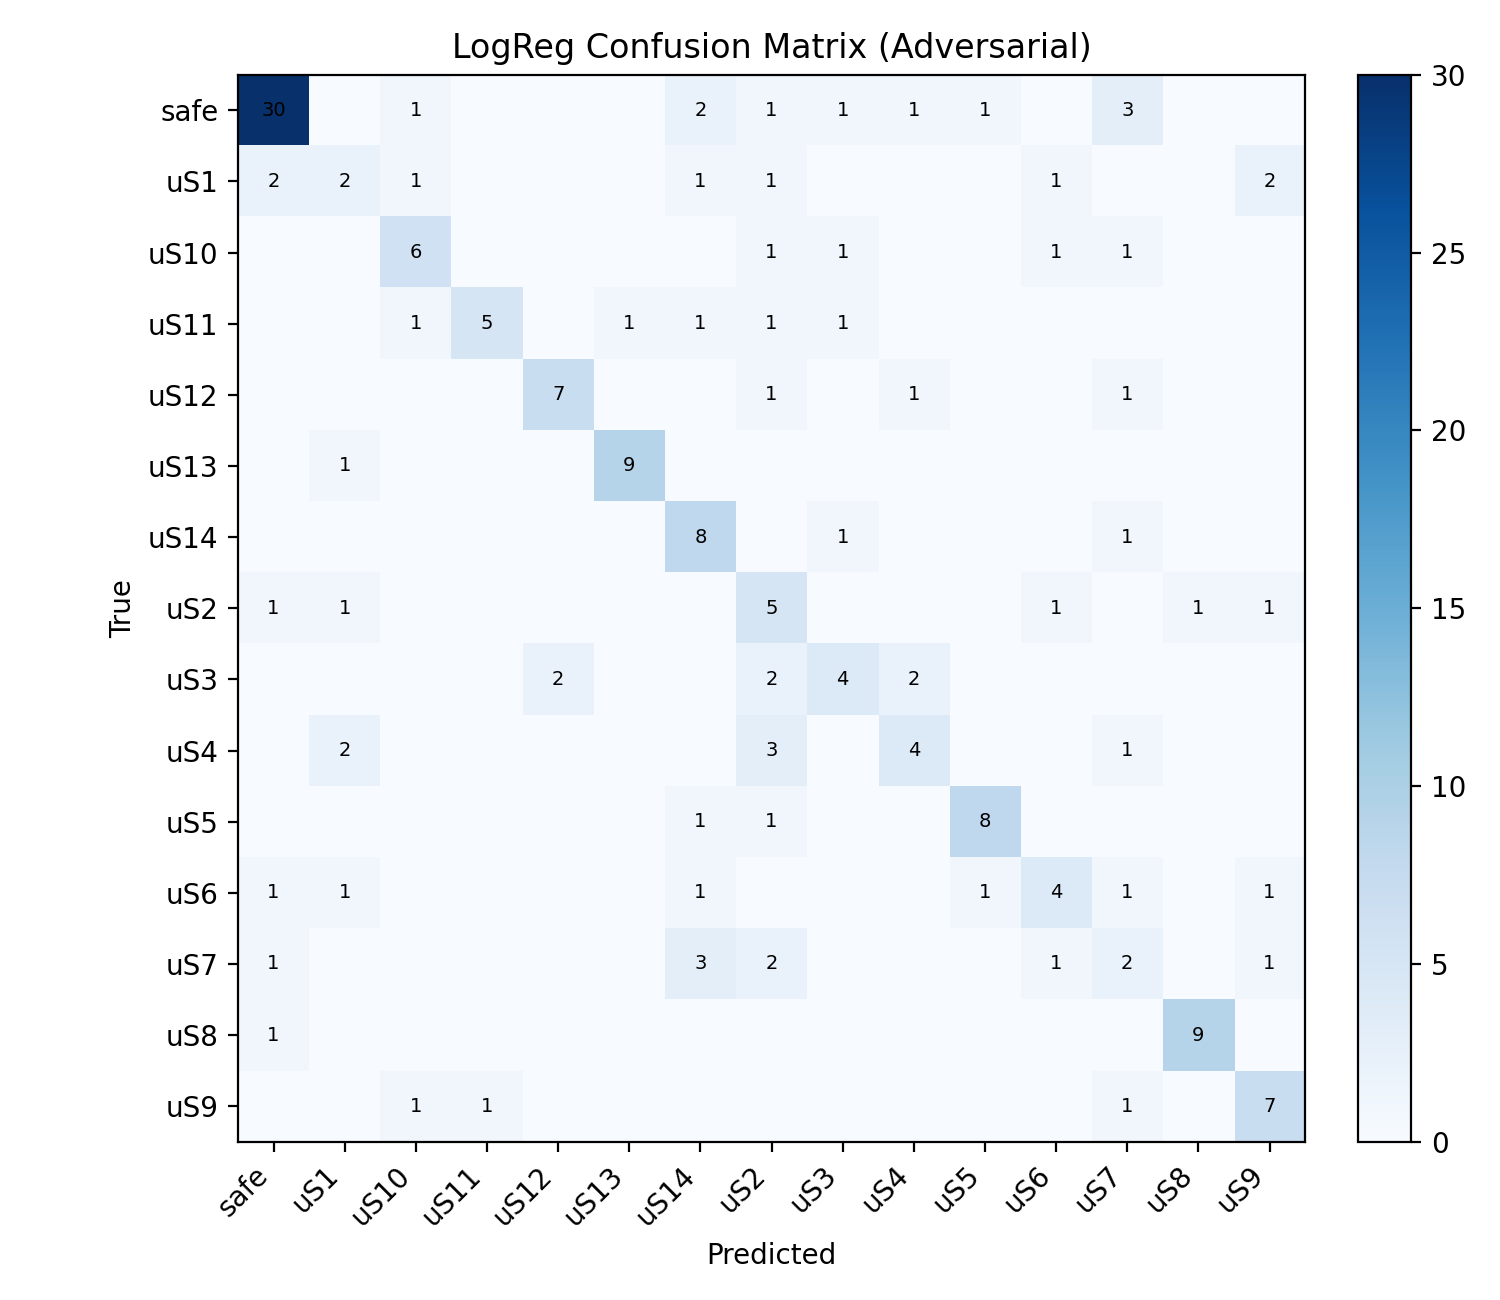
\includegraphics[width=0.8\linewidth]{figures/confusion_logreg_adv.png}
  \caption{Logistic Regression: confusion matrix on adversarial test set}
  \label{fig:cm-adv}
\end{figure}

\begin{figure}[H]
  \centering
  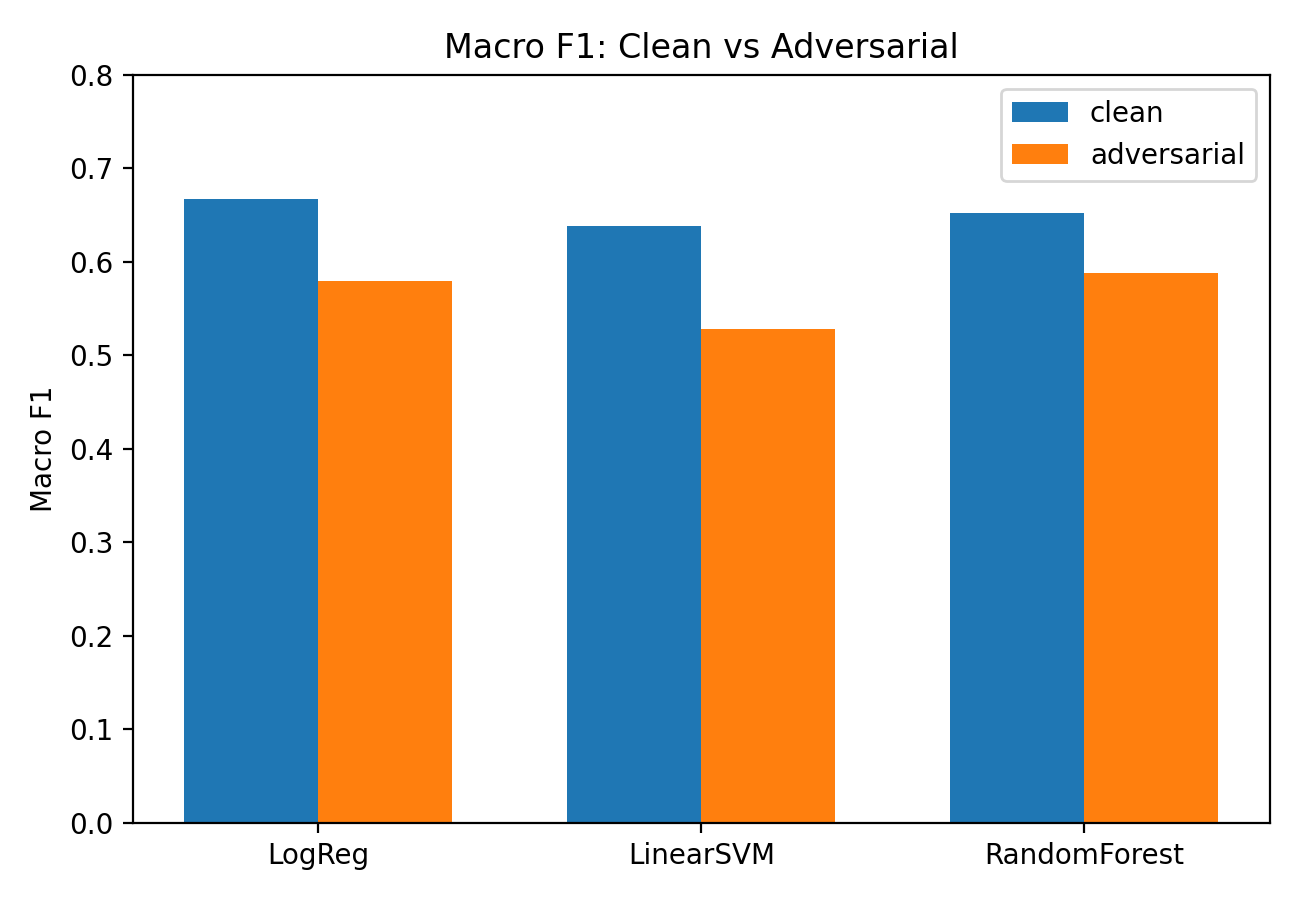
\includegraphics[width=0.8\linewidth]{figures/macro_f1_clean_vs_adv.png}
  \caption{Macro F1 on clean vs adversarial test data (all models)}
  \label{fig:f1-compare}
\end{figure}

\section{Short reflection: what surprised me and what was difficult?}
\subsection*{What surprised me}
\begin{itemize}[leftmargin=*]
\item \textbf{Density fragmentation.} DBSCAN/HDBSCAN label a large fraction as ``noise'' for many reasonable parameters, indicating that the embedding space contains many small/weakly connected groups rather than a few large dense clusters.
\item \textbf{Adversarial sensitivity is moderate, not catastrophic.} About one in five prompts switches K-Means cluster after adversarial edits, and classifier performance drops but not to random---this hints that semantics is partially preserved even under noisy rephrasings.
\end{itemize}

\subsection*{What was difficult}
\begin{itemize}[leftmargin=*]
\item \textbf{Choosing density parameters objectively.} For DBSCAN/HDBSCAN, ``good'' parameters depend on whether we want few outliers (coverage) or many small clusters (resolution). The k-distance plot did not show a sharp elbow, so we relied on a combination of grid search + qualitative inspection.
\item \textbf{Robustness evaluation design.} Comparing clean vs adversarial performance required careful splits and consistent preprocessing (same embedding model, same PCA fit, same label encoding) to avoid accidental leakage.
\end{itemize}

\end{document}
